
\documentclass[a4paper]{article}
\usepackage[margin=1in]{geometry}
\usepackage[english]{babel}
\usepackage[utf8]{inputenc}
\usepackage{amsmath,amsthm,amssymb}
\usepackage{graphicx}
\usepackage{epstopdf}
\usepackage{pdfpages}
\usepackage{float, algorithmic, algorithm2e, program}
\usepackage{tabularx}
\usepackage{longtable}
\usepackage{epstopdf}
\newtheorem{theorem}{Theorem}
\newtheorem{definition}{Definition}[section]

\title{Bathtub Qualitative Reasoning}
\author{Nicola De Cao, Luca Falorsi, Govert Verkes}
\date{\today}

\begin{document}
\maketitle

\section{Base Problem}

\begin{itemize}
\item \textbf{Quantities:}
\begin{itemize}
\item Inflow (of water into the container) $\in [0, +]$
\item Outflow (of water out of the container) $\in [0, +, Max]$
\item Volume (of the water in the container) $\in [0, +, Max]$
\end{itemize}

\item \textbf{Dependencies:}

\begin{itemize}
\item I+(Inflow, Volume): the amount of inflow increases the volume
\item I-(Outflow, Volume): the amount of outflow decreases the volume
\item P+(Volume, Outflow): outflow changes are proportional to volume changes
\item V(Volume(Max), Outflow(Max)): the outflow is at its highest value (Max), when the volume is at it highest value
\item V(Volume(0), Outflow(0)): there is no outflow, when there is no volume
\end{itemize}
\end{itemize}


\begin{figure}[H]
\centering
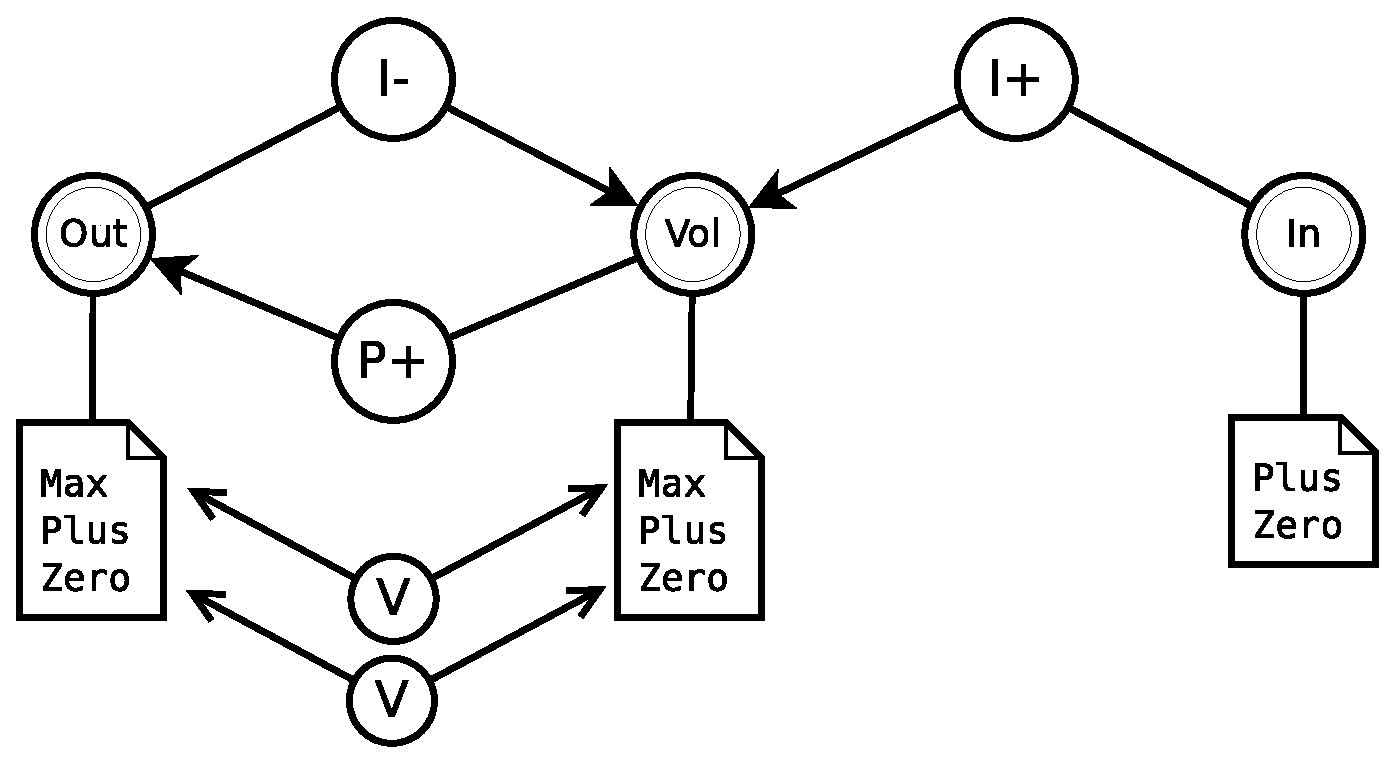
\includegraphics[scale=0.5]{problem1.eps}
\caption{Drawings of the causal model active for the problem}
\end{figure}

\section{Algorithm}
The goal of the algorithm is to construct a state graph based for a specific model and a given starting state. Constructing the state-graph is done iteratively as shown in Algorithm~\ref{alg:computing_state_graph}.
\begin{algorithm}
    result = \{"state": starting\_state, "children": [ ]\}

    processing\_list = [starting\_state]

\While{processing\_list not empty}{
    processing\_state = pop(processing\_list)

    successors = findSuccessors(processing\_state)

    \For{s in succesors}{
        \If{s not in result}{
            add s to result

            add s to processing\_list
        }
        add s as child to processing\_state
    }
}
\caption{Computing the state-graph based on given an starting state. It starts with a given starting state in the processing list, then it computes all the successors of this state and adds all the succesors as children to state that is being processed, as well as adding these succesors to the processing list, but only if a successor was not already processed.}
\label{alg:computing_state_graph}
\end{algorithm}

The core functionality of constructing the state graph is encapsulated in finding all successive states for a given state. The first step in finding the successive states, is propagating over all quantities in the model and computing all possible combinations of new values based on the derivatives. The algorithm for doing this is shown in Algorithm~\ref{alg:propogating_values}.
\begin{algorithm}
new\_states = [ empty\_state ]

    \For{quantity in quantities}{

        p = possible next values for quantity\\
        \ForAll{new\_states}{
            new\_state = pop(new\_states)\\
            \ForAll{p}{
               add new\_state with new possible value for quantity to new\_states
            }
        }
        }
\caption{Propagate over all quantities and modify value based on the derivative}
\label{alg:propogating_values}
\end{algorithm}

After changing the values according to the derivatives for each quantity in the model, we start propagating over all quantities to determine new derivatives based on the influences.
\begin{algorithm}
\For{asd}{
\If{condition}{then-block}
}
\caption{}
\end{algorithm}

\section{State-graph}
The algorithm from the previous section generates a list of states which are unique values of Inflow, Tank and Ouflow and their first derivatives. Each state has a number of reachable states after an amount of time or a change in the state from an external influence. For this problem the only external influence we allow is changing the derivative of the Inflow (which is opening and closing the tap).

In figure \ref{state-graph} shows all possible behaviors of the system described above. Blue nodes are final states, which are states without other reachable states. Other nodes are red and each arrow represents a transition.

\begin{figure}[H]\label{state-graph}
\centering
\includegraphics[width=\textwidth]{result.png}
\caption{Plot of the state-graph}
\end{figure}

\section{Extra Problem}

\begin{itemize}
\item \textbf{Quantities:}
\begin{itemize}
\item Inflow (of water into the container) $\in [0, +]$
\item Outflow (of water out of the container) $\in [0, +, Max]$
\item Volume (of the water in the container) $\in [0, +, Max]$
\item Height (of the water column in the container) $\in [0, +, Max]$
\item Pressure (of the water column at the bottom of the container) $\in [0, +, Max]$
\end{itemize}

\item \textbf{Dependencies:}

\begin{itemize}
\item I+(Inflow, Volume): the amount of inflow increases the volume
\item I-(Outflow, Volume): the amount of outflow decreases the volume
\item P+(Volume, Height): height changes are proportional to volume changes
\item P+(Height, Pressure): pressure changes are proportional to height changes
\item P+(Pressure, Outflow): outflow changes are proportional to pressure changes
\item V(Volume(Max), Height(Max)): the height is at its highest value (Max), when the volume is at it highest value
\item V(Volume(0), Height(0)): there is no height, when there is no volume
\item V(Height(Max), Pressure(Max)): the pressure is at its highest value (Max), when the height is at it highest value
\item V(Height(0), Pressure(0)): there is no pressure, when there is no height
\item V(Pressure(Max), Outflow(Max)): the outflow is at its highest value (Max), when the pressure is at it highest value
\item V(Pressure(0), Outflow(0)): there is no outflow, when there is no pressure
\end{itemize}
\end{itemize}

\begin{figure}[H]
\centering
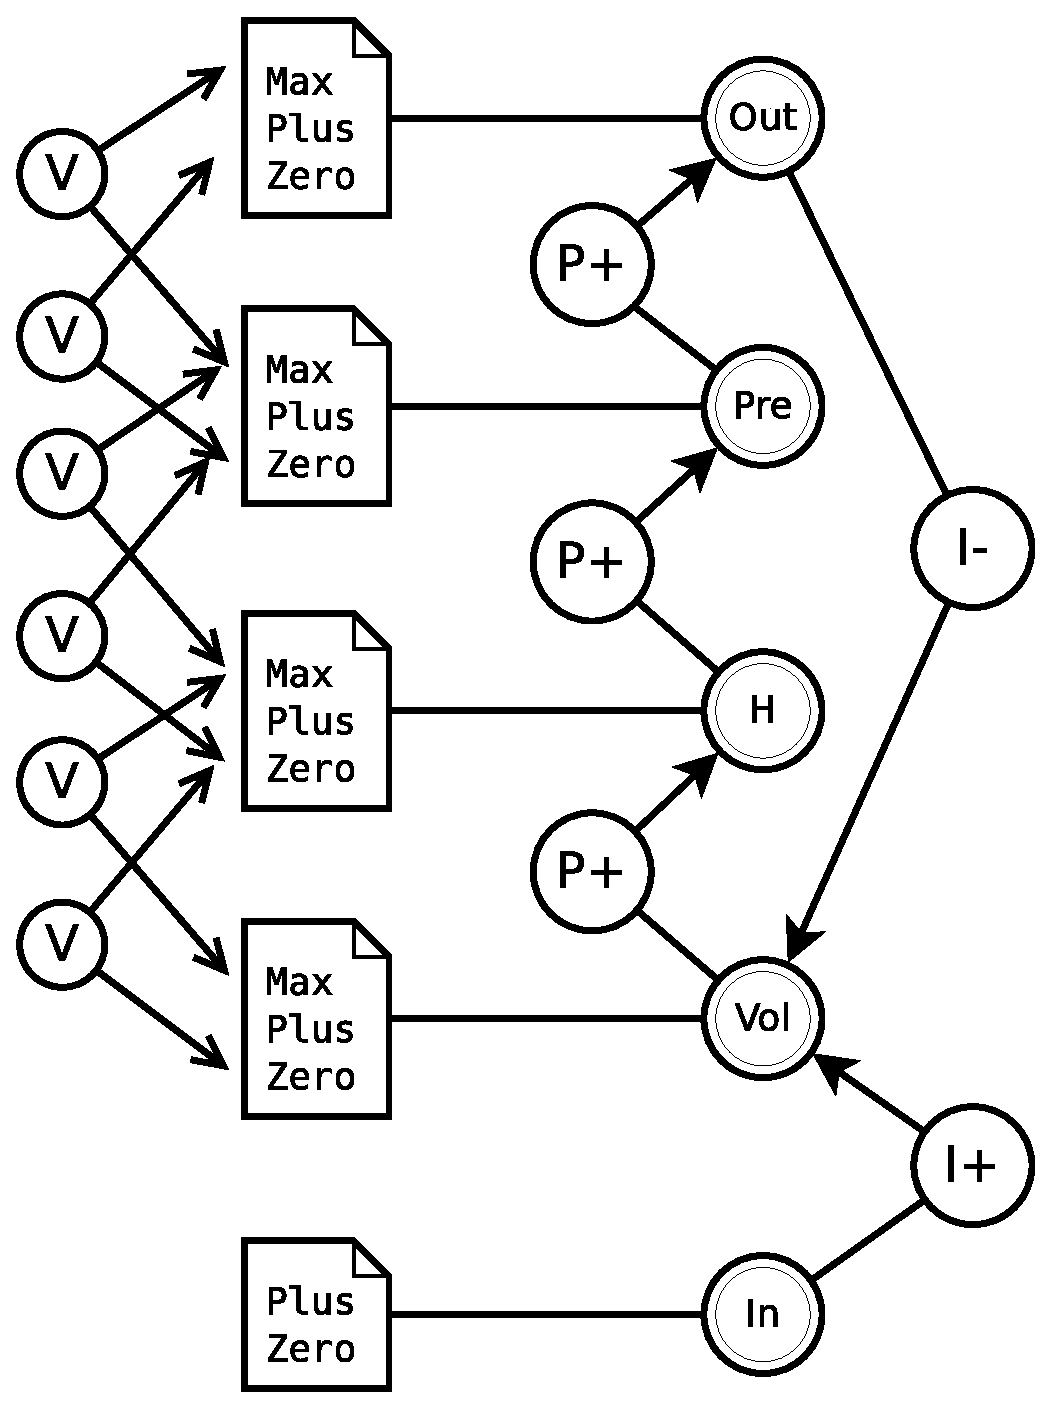
\includegraphics[scale=0.5]{problem_extra.eps}
\caption{Drawings of the causal model active for the extra problem}
\end{figure}


\end{document}

